\section{Homework 3}
\boxed{\text{Sundry: I worked alone.}}
\begin{enumerate}
\setlength{\parskip}{8pt}
\item
    \begin{enumerate}
        \setlength{\parskip}{8pt}
        \item There'd be \boxed{\text{3}} connected components. Note that $n\geq 4$.
        \item For Alice to create a distinct connected component, she would have to remove an edge that is not from a cycle (for otherwise it would still be connected). Therefore she removes 3 edges from some cycles formed from the 10 edges added by Bob, and there would be 7 edges left to remove. Thus at least \boxed{\text{7}} more edges must be removed in order to remove all cycles from the resulting graph.
        \item \boxed{\text{False.}} Counterexample: The complete graph on 3 vertices has $\frac{3(2)}{2}=3$ edges which is less than the $3\cdot2^2=12$ edges of the 3-dimensional hypercube.
        \item The complete graph with $n$ vertices must have $\frac{n(n-1)}{2}$ edges. Each Hamiltonian cycle must consist of $n$ edges. Therefore the required number of such cycles is \boxed{\frac{n-1}{2}}.
    \item We have two such hamiltonian cycles in the set: $\{(0, 1),(1, 2),(2, 3),(3, 4),(4, 0)\}$, and $\{(0, 2),(2, 4),(4, 1),(1, 3),(3, 0)\}$.
    \end{enumerate}
    
    \item
    \begin{enumerate}
        \setlength{\parskip}{8pt}
        \item \boxed{\text{No,}} because an Eulerian tour must have only even degree vertices, yet in the graph shown vertices 3 and 7 have an odd number of edges.
        \item \boxed{\text{Yes.}} There are multiple Eulerian walks starting from/ending at vertices 3 and 7. One such walk is $(3,1,2,4,3,2,6,1,4,8,1,7,6,8,7)$.
        \item The condition for an Eulerian walk in an undirected graph is that every vertex except for two (the starting and ending vertices) must have even degree, and the two exceptions must have odd degree. This is because for the starting and ending vertex, there must be one unpaired edge (since the walk leaves the starting vertex but doesn't end on it, and since the walk arrives at the ending vertex but doesn't start on it), whereas for the vertices in between, each incident edge must be paired.
    \end{enumerate}
    \item We first prove that \textbf{if} a graph is bipartite then it cannot have any tours of odd length. Let $G$ be a bipartite graph with its vertices split into two sets $A$ and $B$ such that there exist no edges within $A$ and no edges within $B$. Then any tour in $G$ must begin and end on the same vertex, and therefore must begin and end in the same set $A$ or $B$. Suppose for the sake of contradiction that there exists a tour $T$ of odd length. WLOG, say the first vertex in $T$ is in $A$. Note that every time we traverse an edge in $T$, we alternate between $A$ and $B$ since there exists no edges within $A$ nor within $B$. Then if we traverse an odd number of edges, we must end up in $B$ (assuming we started in $A$). But then the tour $T$ cannot be closed, a contradiction. Thus any bipartite graph cannot have tours of odd length.
    
    Now we prove the \textbf{converse}, which is more complex to prove. Say we have a graph $G$ with no odd tours. Then $G$ can only have tours of even length. Note that since every cycle is a tour, this implies that $G$ can only have cycles of even length. Therefore if we can prove that ($G$ has no cycles of odd length) implies ($G$ is bipartite), we are done. We will describe an algorithm for coloring every vertex red or blue such that no two red vertices nor any two blue vertices share an edge. 
    
    First, pick an arbitrary vertex $v$ of $G$ and color it red. Then every step of the algorithm consists taking a colored vertex and coloring the adjacent vertices the opposite color (if red then blue, if blue then red). Now we will prove that this algorithm will always color the vertices such that no two adjacent vertices are the same color. We will claim that at every step of this algorithm, \textbf{(i)} the length of any path (containing only colored vertices) between two colored vertices of the same color must be even, whereas \textbf{(ii)} the length of any path (also containing only colored vertices) between two colored vertices of different color must be odd. 
    
    At the beginning of the algorithm, note that we color one vertex red, and both of these conditions are satisfied. Now, at every subsequent step, coloring a new vertex $v'$ adjacent to an already colored vertex $v$ will extend any pre-existing path from $v$ by one, therefore flipping the parity of the path but also flipping the color of the endpoint. Therefore every new path consisting of colored vertices must satisfy conditions \textbf{(i)} and \textbf{(ii)}. Now, for some subsequent step of the algorithm say we took any vertex and called it $a$. WLOG let $a$ be colored red. Then if at this step we were to color a vertex $b$ adjacent to $a$ such that there exists an already colored path from $a$ to $b$ other than the edge connecting them, it must be true that $a$ and $b$ are different colors. In other words, any colored cycle that we generate would satisfy the condition that no two adjacent vertices within the cycle are of the same color. This is because $a$ and $b$ are connected by an edge, and since the colored cycle starting at $a$ and going through $b$ must have even length, we know that the colored path from $a$ to $b$ that is not the edge connecting $a$ and $b$ must have odd length. Then by condition \textbf{(ii)}, $a$ and $b$ must be of different colors. Thus, given a graph with no odd cycles, this algorithm will never produce two adjacent vertices of the same color. Then at the end of the algorithm we can organize the red vertices into one group and the blue into another group and we have a bipartite graph. $\square$
    
    \item 
        \textit{Note: I used tikz package to draw these graphs, if you don't believe me then email me (albertczhang@berkeley.edu) and I'll send you my tex file}
    \begin{enumerate}
        \setlength{\parskip}{8pt}
        \item 1-D Hypercube:
        
        \begin{tikzpicture}
            \node (a) at (0,0){``0''};
            \node (b) at (2,0){``1''};
            \draw (a) -- (b);
        \end{tikzpicture}
        
        2-D Hypercube:
        
        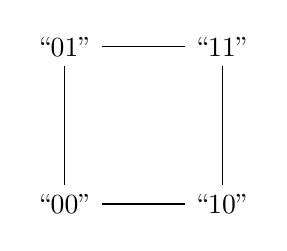
\begin{tikzpicture}
            \node (a) at (0, 0){``00''};
            \node (b) at (0, 2){``01''};
            \node (c) at (2, 0){``10''};
            \node (d) at (2, 2){``11''};
            \draw (a) -- (b) -- (d) -- (c) -- (a);
        \end{tikzpicture}
        
        3-D Hypercube: (on next page)
        
        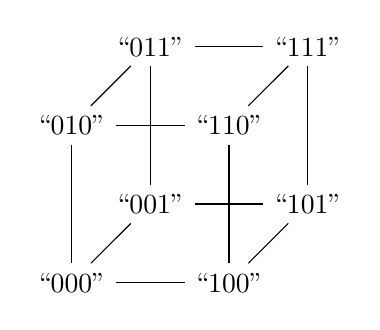
\begin{tikzpicture}
            \node (a) at (0, 0){``000''};
            \node (b) at (2, 0){``100''};
            \node (c) at (2, 2){``110''};
            \node (d) at (0, 2){``010''};
            \node (e) at (1, 1){``001''};
            \node (f) at (3, 1){``101''};
            \node (g) at (3, 3){``111''};
            \node (h) at (1, 3){``011''};
            \draw (a) -- (b) -- (c) -- (d) -- (a);
            \draw (e) -- (f) -- (g) -- (h) -- (e);
            \draw (a) -- (e);
            \draw (b) -- (f);
            \draw (c) -- (g);
            \draw (d) -- (h);
        \end{tikzpicture}
        
        \item We will show inductively that for any $n\geq1$, the $n$ dimensional hypercube can be split into two disjoint sets (which we'll call set $A$ and $B$) of vertices of equal cardinality such that the graph is bipartite.
        
        \textit{Base Case:} When $n=1$, we have two vertices connected by an edge. The graph is obviously bipartite as we can put each vertex in its own group, with no edges within each group, and each group has an equal number of vertices (i.e. one).
        
        \textit{Inductive Hypothesis:} Suppose that for some $n\geq1$, the $n$ dimensional hypercube can be split into two disjoint sets of vertices of equal cardinality (call these two sets $A$ and $B$), such that its graph is bipartite. 
        
        \textit{Inductive Step:} To form the $n+1$ dimensional hypercube, we can take two $n$ dimensional hypercubes and draw an edge between each corresponding vertex. Say the $n$ dimensional hypercube is bipartite with disjoint sets of vertices $A$ and $B$, both with $2^{n-1}$ vertices. Then to form the $n+1$ dimensional hypercube, we create mirrored sets $A'$ and $B'$ of a duplicate $n$ dimensional hypercube such that we only draw additional edges between corresponding vertices in $A$ and $A'$, and between corresponding vertices in $B$ and $B'$. Then we can divide the $n+1$ dimensional hypercube into two sets $A\cup B'$ and $B\cup A'$. There cannot exist an edge within $A$, $B$, $A'$, or $B'$ by the inductive hypothesis, and furthermore there cannot exist an edge between a vertex in $A$ and a vertex in $B'$ (nor between a vertex in $B$ and a vertex in $A'$) by the method in which we constructed and grouped our vertices in the $n+1$ dimensional hypercube. Therefore the $n+1$ dimensional hypercube is also bipartite, and we can split it into two disjoint sets of vertices of equal cardinality ($|A|=|B|=|A'|=|B'|$, therefore $|A\cup B'|=|B\cup A'|$ since all these sets are disjoint). $\square$
    \end{enumerate}
    
    \item
    \begin{enumerate}
        \setlength{\parskip}{8pt}
        \item Let $V$ be the total number of vertices, $E$ the total number of edges, and $F$ the total number of faces. Then since each edge is counted twice for each bordering face, and each face has 3 edges, then we have that $3F=2E$. Then substituting into Euler's formula we have $V=\frac{E}{3}+2$ or $E=3V-6$. The sum of the "charges" is equal to $\sum_v{(6-\text{degree}{(v)})}=6V-2E$, since each edge is counted twice in the sum of the degrees of the vertices. Then combining what we have above we get $6V-2E=6V-2(3V-6)=\boxed{12}$.
        
        \item The charge of a degree 5 vertex is \boxed{1}, and the charge of a degree 6 vertex is \boxed{0}.
        
        \item After discharging all the degree 5 vertices, the only way for a degree 5 vertex to retain a positive remaining charge is for it to be adjacent to at least one other vertex of degree less than or equal to 6 (any vertex of degree $>6$ would have negative charge). Then, under this assumption, the proof follows since either condition (1), (2), or (3) must be true.
        
        \item After discharging, the sum of the charges of all the vertices should remain unchanged, since discharging \textit{transfers} portions of charge from degree 5 vertices to other negatively charged vertices. Thus the total charge must remain 12, and there must exist at least one vertex with positive charge (if all the charges were negative, they wouldn't be able to sum to 12).
        
        Since all degree 5 vertices are "fully" discharged to 0, no degree 5 vertex can have positive charge. The only possible degree of a vertex that goes from negative to positive charge is 7. This is because a degree 7 vertex can receive up to $7\cdot\frac{1}{5}=\frac{7}{5}$ positive charge from surrounding degree 5 vertices, and this is enough to convert its charge of -1 to a positive charge. For any vertex of degree $d>7$, $d\cdot\frac{1}{5}=\frac{d}{5}<|6-d|$, i.e. the surrounding charges from degree 5 vertices is not enough to convert the vertex to a positive degree. Also, degree 6 vertices are unaffected but have 0 charge. Thus the only possible degrees of any positively charged vertex after discharging are \boxed{\text{1, 2, 3, 4, and 7}}.
        
        \item If there exists a degree 7 vertex with positive charge, then it must have \boxed{\text{6 or 7}} adjacent degree 5 vertices, since it's original charge was -1, and it takes at least 6 one-fifth charges to reach a positive charge.
        
        \item Call the degree 7 vertex $a$, and its 7 neighbors $b_1,b_2,b_3,b_4,b_5,b_6,b_7$ in clockwise order. Then, since the graph is triangulated and planar, there must exist an edge between $b_i$ and $b_{i+1}$ for $1\leq i\leq 7$ (since any face consisting of $b_i$, $b_{i+1}$, and $a$ can only have 3 edges, and 2 of the 3 are already drawn) where $i$ and $i+1$ are taken mod 7. Therefore, since at least 6 of the $b_i$ are degree 5, there must exist an edge between two degree 5 vertices, or an edge between a degree 5 vertex and a degree 6 vertex.
        
        \item Let $T$ be any triangulated planar graph. Then from part (a), we know that the total charge of $T$ must be 12. Now, if we "discharge" all degree 5 vertices in $T$, then one of two things can result: (i) there exists a degree 5 vertex with positive charge, or (ii) there exists no degree 5 vertex of positive charge. 
        
        If (i) is true, then by (c) there must exist two degree 5 vertices which are adjacent, satisfying condition (2). 
        
        On the other hand, if (ii) is true, then by (d) there must exist a vertex of degree either 1, 2, 3, 4, or 7. If the vertex has degree 1, 2, 3, 4, condition (1) is satisfied. If the vertex has degree 7, then by parts (e) and (f), we know that there must exist two degree 5 vertices which are adjacent to each other, satisfying condition (2) or condition (3).
        
        Thus we have shown that no matter what either condition (1) or condition (2) or condition (3) will be satisfied for triangulated planar graphs. $\square$
        
    \end{enumerate}
    
\end{enumerate}